\documentclass[11pt,a4j,fleqn]{jarticle}
\usepackage{amsmath,amsthm,amssymb}
\usepackage[dvipdfmx]{graphicx}

\title{包絡線定理レポート}
\author{大野 嵩侃}
\date{2014年6月7日}


\begin{document}

\maketitle

\section{はじめに}



\section{包絡線定理}

包絡線定理の解説を書く.

数式(番号なし)の例
\[
f(x, t) = t x - t^2
\]


数式(番号つき)の例
\begin{equation}
f(x, t)  = -(t - \frac{x}{2})^2 + \frac{x^2}{4} \label{eq:square}
\end{equation}

数式(番号つき)の例(高さが調整されたカッコ)
\begin{equation}
f(x, t) = -\left(t - \frac{x}{2}\right)^2 + \frac{x^2}{4} \label{eq:square-2}
\end{equation}



数式番号の引用の例:
平方完成の式\eqref{eq:square}より...

\begin{figure}
 \centering
 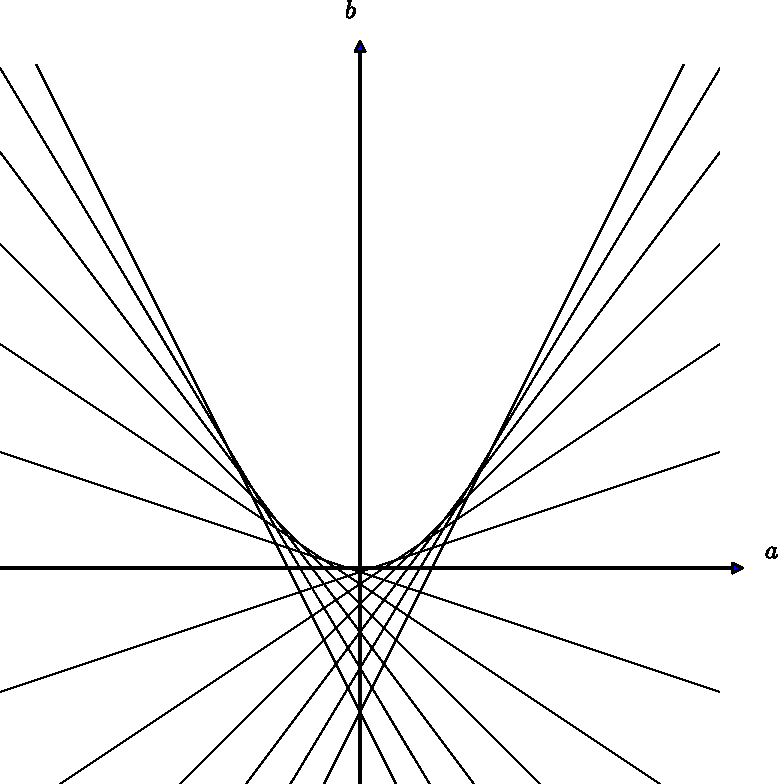
\includegraphics{envelope0.pdf}
 \caption{1つ目の図の表示}
 \label{fig:1}
\end{figure}

\begin{figure}
 \centering
 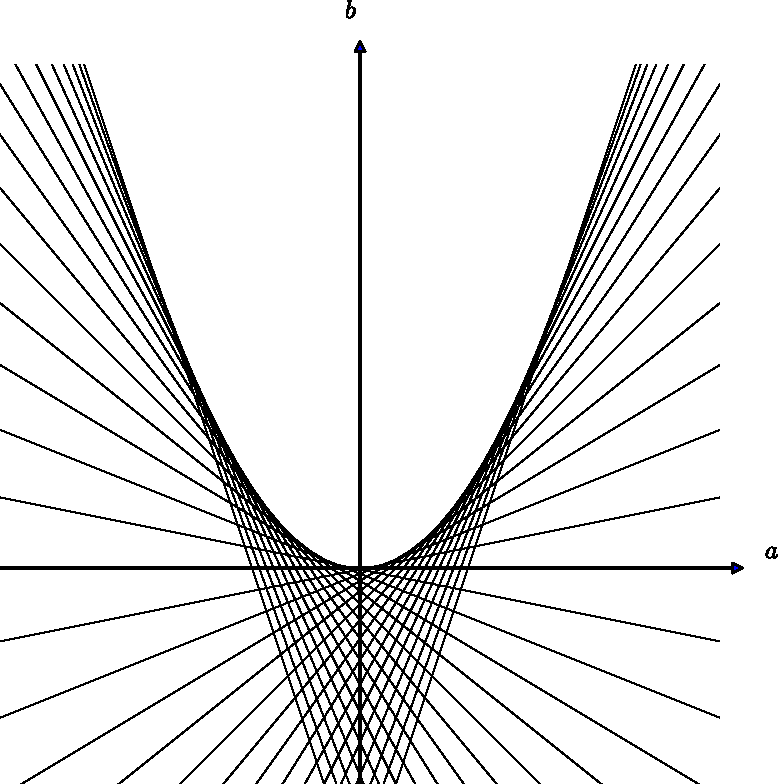
\includegraphics{envelope1.pdf}
 \caption{2つ目の図の表示}
 \label{fig:2}
\end{figure}



引用の例:尾山・安田\cite{OyamaYasuda11}.


\subsection{サブセクションのタイトル}

必要ならサブセクションを作る.


\newpage
\section{Pythonプログラム}
\subsection{コード}
\begin{quote}
\begin{verbatim}
1  	from __future__ import division
2  	from numpy import linspace
3  	from numpy import fabs
4  	from numpy import array
5  	from mpl_toolkits.axes_grid.axislines import SubplotZero
6  	import matplotlib.pyplot as plt
7  	
8  	
9  	def f(x, a):
10 	    return a*x-x**2
11 	p = -3
12 	q = 3
13 	n = 12
14 	a_min = -10
15 	a_max = 10
16 	y_min = -6
17 	y_max = y_min+a_max-a_min
18 	plt.figtext(0.85, 0.35, '$a$')
19 	plt.figtext(0.5, 0.95, '$b$')
20 	fig = plt.figure(1)
21 	ax = SubplotZero(fig, 111)
22 	fig.add_subplot(ax)
23 	ax.axhline(linewidth=1.0, color="black")
24 	ax.axvline(linewidth=1.0, color="black")
25 	ax.set_xticks([])
26 	ax.set_yticks([])
27 	ax.set(aspect=1)
28 	for direction in ["xzero", "yzero"]:
29 	    ax.axis[direction].set_axisline_style("-|>")
30 	    ax.axis[direction].set_visible(True)
31 	for direction in ["left", "right", "bottom", "top"]:
32 	    ax.axis[direction].set_visible(False)
33 	plt.ylim(ymin=y_min)
34 	plt.ylim(ymax=y_max)
35 	a = array([a_min, a_max])
36 	for i in range(n):
37 	    r = p+(q-p)*i/(n-1)
38 	    b = f(r, a)
39 	    ax.plot(a, b, 'k', linewidth=0.5, alpha=1)'
40 	plt.show()
\end{verbatim}
\end{quote}

\subsection{コードの解説}
\begin{quote}
\begin{verbatim}
1~6行目:必要な機能を各モジュールからインポートしています。
9, 10行目:f(x, a)を定義しています。xにいくつかの値を代入し、最終的にa-bグラフを求めます。
\end{verbatim}
\end{quote}


\begin{thebibliography}{0}
\bibitem{OyamaYasuda11}
尾山大輔・安田洋祐「経済学で出る包絡線定理」『経済セミナー』2011年10・11月号.
\end{thebibliography}

\end{document}
